\section{Concorrenza}

Un criterio per classificare i sistemi di gestione di basi di dati è il numero di utenti che possono
usare il sistema concorrentemente. Un sistema è \textbf{singolo-utente} se può essere usato da al più un
utente alla volta ed è \textbf{multiutente} se molti utenti possono usarlo contemporaneamente; la maggior
parte dei sistemi di gestione di basi di dati è del secondo tipo.\\
Se il sistema di calcolo ha più CPU allora è possibile il simultaneo processamento di due
programmi da parte di due diverse CPU; tuttavia la maggior parte della teoria del controllo della
concorrenza nelle basi di dati è stata sviluppata per sistemi di calcolo con una sola CPU. In tali
sistemi i programmi sono eseguiti concorrentemente in modo \emph{interleaved}, ovvero interfogliato: la CPU
può eseguire un solo programma alla volta, tuttavia il sistema operativo permette di eseguire alcune
istruzioni di un programma, sospendere quel programma, eseguire istruzioni di un altro programma
e quindi ritornare ad eseguire istruzioni del primo. In tal modo l'esecuzione concorrente dei
programmi è interleaved; ciò consente di tenere la CPU occupata quando un programma deve
effettuare operazioni di I/O.\\
\subsection{Scheduling di transazioni}
In un sistema di gestione di basi di dati multiutente la principale risorsa a cui i vari programmi
accedono concorrentemente è la base di dati. L'esecuzione di una parte di un programma che
rappresenta un'unità logica di accesso o modifica del contenuto della base di dati è detta
transazione. Ci sono sistemi (ad esempio le basi di dati statistici) in cui gli utenti effettuano solo
interrogazioni ma non modifiche; in tali sistemi l'esecuzione concorrente di più transazioni non crea
problemi. Al contrario nei sistemi in cui vengono effettuate da più utenti sia operazioni di lettura
che di scrittura (un tipico esempio di sistemi di questo tipo è costituito dai sistemi per la
prenotazione di posti sui voli) l'esecuzione concorrente di più transazioni può provocare problemi
se non viene controllata in qualche modo.\\
Prima di esaminare alcuni dei problemi che possono sorgere quando l'esecuzione concorrente di più
transazioni non è controllata, introduciamo il concetto di \textbf{schedule} (piano di esecuzione) di un
insieme di transazioni.
\begin{defn}
Dato un insieme $T$ di transazioni, uno \textbf{schedule} $S$ di $T$ è un ordinamento delle
operazioni nelle transazioni in $T$ tale che, per ogni transazione $t$ in $T$, se $o_1$ e $o_2$ sono due operazioni
in $t$ tali che $o_1$ precede $o_2$ in $t$ allora $o_1$ precede $o_2$ in $S$.
\end{defn}
In altre parole uno schedule deve \emph{conservare l'ordine} che le operazioni hanno all'interno delle singole 
transazioni. Qualsiasi schedule ottenuto permutando le transazioni in $T$ è detto \emph{seriale}.
Consideriamo le seguenti transazioni

\begin{multicols}{2}  
 \begin{tabular}{|l|}
   \hline
   $t_1$\\
   \hline
   read(X)\\ 
   $X\vcentcolon=X-N$\\ 
   write(X)\\ 
   read(Y)\\
   $Y\vcentcolon=Y+N$\\
   write(Y)\\
   \hline
  \end{tabular} 
  
 \begin{tabular}{|l|}
  \hline
   $t_2$\\
   \hline
   read(X)\\ 
   $X\vcentcolon=X+M$\\ 
   write(X)\\
   \\
   \\
   \hline
  \end{tabular}\\
 \end{multicols}
 
 e i seguenti schedule di $\{t_1,t_2\}$:

 \begin{multicols}{2}  
 \begin{tabular}{|l|l|}
 \hline
 $t_1$ & $t_2$\\
 \hline
   read(X) & \\ 
   $X\vcentcolon=X-N$ & \\ 
   & read(X)\\
   & $X\vcentcolon=X+M$\\ 
   write(X) &\\ 
   read(Y) &\\
   & write(X)\\
   $Y\vcentcolon=Y+N$ &\\
   write(Y)&\\
   \hline
  \end{tabular}
  
  \begin{tabular}{|l|l|}
   \hline
   $t_1$ & $t_2$\\
   \hline
   read(X) & \\ 
   $X\vcentcolon=X-N$ & \\ 
   write(X) &\\ 
   & read(X)\\
   & $X\vcentcolon=X+M$\\ 
   & write(X)\\
   read(Y) &\\
   $t_1$ fallisce &\\
 
   \hline
  \end{tabular}
  
  
 \end{multicols}

Nel primo caso l'aggiornamento di $X$ prodotto da $t_1$ viene perso in quanto $t_2$ legge il valore di $X$
prima che l'aggiornamento prodotto da $t_1$ sia stato reso permanente. Nel secondo caso $t_2$ legge e
aggiorna il valore di $X$ dopo che l'aggiornamento prodotto da $t_1$ è stato reso permanente, ma prima
che venga ripristinato il vecchio valore di $X$ in conseguenza del fallimento di $t_1$.\\

Consideriamo ora una transazione $t_3$ che somma i valori di $X$ e di $Y$. Il seguente schedule di
$\{t_1, t_3\}$ fa sì che la somma prodotta da $t_3$ sia la somma del valore di $X$ dopo che $X$ è stato
aggiornato da $t_1$ e del valore di $Y$ prima che sia stato aggiornato da $t_1$.
\begin{center}
  \begin{tabular}{|l|l|}
   \hline
   $t_1$ & $t_3$\\
   \hline
   & $somma\vcentcolon=0$\\
   read(X) & \\ 
   $X\vcentcolon=X-N$ & \\ 
   write(X) &\\ 
   & read(X)\\
   & $somma\vcentcolon=somma + X$\\ 
   & read(Y)\\
   & $somma\vcentcolon= somma + Y$\\
   read(Y) &\\
   $Y\vcentcolon=Y+N$ &\\
   write(Y)&\\
   \hline
  \end{tabular}
\end{center}
In tutti e tre i casi visti siamo portati a considerare gli schedule non corretti in quanto i valori
prodotti non sono quelli che si avrebbero se le due transazioni fossero eseguite nel modo ``naturale''
cioè sequenzialmente.\\
In generale possiamo osservare che l'esecuzione naturale e, quindi, intuitivamente corretta di un
insieme di transazioni è quella \emph{sequenziale}; la possibilità di eseguire concorrentemente un insieme
di transazioni, come si è detto, è introdotta nei sistemi per motivi di efficienza. Pertanto tutti gli
schedule seriali sono corretti e uno schedule non seriale è corretto se è \emph{serializzabile}, cioè se è
``\textbf{equivalente}'' ad uno schedule seriale. Sorge quindi la necessità di definire un concetto di
equivalenza di schedule.\\
La più semplice definizione di equivalenza potrebbe essere basata sul confronto del risultato: due
schedule sono equivalenti se producono lo stesso stato finale. Tale definizione non è però
soddisfacente in quanto due schedule potrebbero produrre lo stesso stato finale solo per alcuni
valori iniziali. Consideriamo ad esempio le due transazioni 
\begin{multicols}{2}  
 \begin{tabular}{|l|}
   \hline
   $t_1$\\
   \hline
   read(X)\\ 
   $X\vcentcolon=X+5$\\ 
   write(X)\\ 
   \hline
  \end{tabular}

  \begin{tabular}{|l|}
  \hline
   $t_2$\\
   \hline
   read(X)\\ 
   $X\vcentcolon=X*1.5$\\ 
   write(X)\\
   \hline
  \end{tabular}

 \end{multicols}

 e i seguenti schedule di $\{t_1,t_2\}$:
\begin{multicols}{2}  
 \begin{tabular}{|l|l|}
 \hline
 $t_1$ & $t_2$\\
 \hline
   read(X) & \\
   & read(X)\\
   $X\vcentcolon=X+5$ & \\ 
   & $X\vcentcolon=X*1.5$\\
   & write(X)\\ 
   write(X) &\\ 
   \hline
  \end{tabular}

  \begin{tabular}{|l|l|}
   \hline
   $t_1$ & $t_2$\\
   \hline
   read(X) & \\
   & read(X)\\
   & $X\vcentcolon=X*1.5$\\
   $X\vcentcolon=X+5$ & \\ 
   write(X) &\\   
   & write(X)\\
   \hline
  \end{tabular}
 \end{multicols}
 
Tali schedule producono gli stessi valori solo se il valore iniziale di $X$ è $10$; ma producono valori
diversi in tutti gli altri casi. Problemi di questo tipo potrebbero essere evitati sfruttando proprietà
algebriche che garantiscano che il risultato sia lo stesso indipendentemente dai valori iniziali delle
variabili; tuttavia tale soluzione richiederebbe dei costi inaccettabili (che non sono giustificati dallo
scopo che si vuole raggiungere). Pertanto si fa l'assunzione più restrittiva che due valori sono
uguali solo se sono prodotti da esattamente la stessa sequenza di operazioni. Quindi, ad esempio,
date le due transazioni

\begin{multicols}{2}  
 \begin{tabular}{|l|}
   \hline
   $t_1$\\
   \hline
   read(X)\\ 
   $X\vcentcolon=X+N$\\ 
   write(X)\\ 
   \hline
  \end{tabular}



  \begin{tabular}{|l|}
  \hline
   $t_2$\\
   \hline
   read(X)\\ 
   $X\vcentcolon=X-M$\\ 
   write(X)\\
   \hline
  \end{tabular}

 \end{multicols}

 e i due schedule:
\begin{multicols}{2}  
 \begin{tabular}{|l|l|}
 \hline
 $t_1$ & $t_2$\\
 \hline
   read(X) & \\
   $X\vcentcolon=X+N$&\\ 
   write(X)&\\ 
   &read(X)\\ 
   &$X\vcentcolon=X-M$\\ 
   &write(X)\\
   \hline
  \end{tabular}

  \begin{tabular}{|l|l|}
   \hline
   $t_1$ & $t_2$\\
   \hline
   &read(X)\\ 
   &$X\vcentcolon=X-M$\\ 
   &write(X)\\
   read(X) & \\
   $X\vcentcolon=X+N$&\\ 
   write(X)&\\ 
   \hline
  \end{tabular}
 \end{multicols}
 
non sono considerati equivalenti.\\

Oltre alla definizione di equivalenza, un altro elemento che ha influenza sulla complessità del
problema di decidere se uno schedule è serializzabile (cioè se è equivalente ad uno schedule seriale)
è costituito dal fatto che il valore calcolato da una transazione per ogni dato sia \emph{dipendente} o meno
dal vecchio valore di quel dato. Nel primo caso il problema della serializzabilità può essere risolto
in tempo polinomiale con un semplice algoritmo su grafi; nel secondo caso il problema risulta
essere \emph{NP-completo}.\\
Nella pratica è difficile testare la serializzabilità di uno schedule. Infatti l'ordine di esecuzione delle
operazioni delle diverse transazioni è determinato in base a diversi fattori: il carico del sistema,
l'ordine temporale in cui le transazioni vengono sottomesse al sistema e le loro priorità. Pertanto è
praticamente impossibile determinare in anticipo come le operazioni saranno interleaved, cioè in
quale ordine verranno eseguite; d'altra parte, se prima si eseguono le operazioni e poi si testa la
serializzabilità dello schedule, i suoi effetti devono essere annullati se lo schedule risulta non
serializzabile. Inoltre quando le transazioni vengono sottomesse al sistema in modo continuo è
difficile stabilire quando uno schedule comincia e quando finisce. Quindi l'approccio seguito nei
sistemi è quello di determinare metodi che garantiscano la serializzabilità di uno schedule
eliminando così la necessità di dover testare ogni volta la serializzabilità di uno schedule. Uno di
tali metodi consiste nell'imporre dei protocolli, cioè delle regole, alle transazioni in modo da
garantire la serializzabilità di ogni schedule. Questi protocolli usano tecniche di \emph{locking} (cioè di
controllo dell'accesso ai dati) per prevenire l'accesso concorrente ai dati. Altri metodi di controllo
usano i \textbf{timestamp} delle transazioni, cioè degli identificatori delle transazioni che vengono generati
dal sistema e in base ai quali le operazioni delle transazioni possono essere ordinate in modo da
assicurare la serializzabilità.

\subsection{Item}
Tutte le tecniche per la gestione della concorrenza richiedono che la base di dati sia partizionata in
item, cioè in unità a cui l'accesso è controllato. Le dimensioni degli item devono essere definite in
base all'uso che viene fatto della base di dati in modo tale che in media una transazione acceda a
pochi item. Ad esempio se la transazione tipica su una base di dati relazionale è la ricerca di una
tupla mediante un indice, è appropriato trattare le tuple come item; se invece la transazione tipica
consiste nell'effettuazione di un join di due relazioni, è opportuno considerare le relazioni come
item. Le dimensioni degli item usate da un sistema sono dette la sua granularità. Una granularità
grande permette una gestione efficiente della concorrenza; una piccola granularità può invece
sovraccaricare il sistema, ma consente l'esecuzione concorrente di molte transazioni.

\subsection{Tecniche di locking per il controllo della concorrenza}
Queste tecniche fanno uso del concetto di lock. Un \textbf{lock} è un privilegio di accesso ad un singolo
item. In pratica è una variabile associata all'item il cui valore descrive lo stato dell'item rispetto alle
operazioni che possono essere effettuate su di esso. Un lock viene richiesto da una transazione
mediante un'operazione di locking e viene rilasciato mediante un'operazione di unlocking; fra
l'esecuzione di un'operazione di locking su un certo item $X$ e l'esecuzione di un'operazione di
unlocking su $X$ diciamo che la transazione mantiene un lock su $X$. Sono stati studiati diversi tipi di
lock; in ogni caso si assume che una transazione debba effettuare un'operazione di locking ogni
volta che deve leggere o scrivere un item e che l'operazione agisca come primitiva di
sincronizzazione, cioè se una transazione richiede un lock su un item su cui un'altra transazione
mantiene un lock, la transazione non può procedere finchè il lock non viene rilasciato dall'altra
transazione. Inoltre si assume che ciascuna transazione rilascia ogni lock che ha ottenuto. Uno
schedule è detto legale se obbedisce a queste regole.

\subsubsection{Lock binario}
Un \textbf{lock binario} può assumere solo due valori \emph{locked} e \emph{unlocked}. Le transazioni 
fanno uso di due operazioni \emph{lock(X)} e \emph{unlock(X)}; la prima serve per richiedere l'accesso
all'item $X$, la seconda per rilasciare l'item $X$ consentendone l'accesso ad altre transazioni. Se una 
transazione richiede l'accesso ad un item $X$ mediante un lock(X) e il valore della variabile è locked 
la transazione viene messa in attesa, altrimenti viene consentito alla transazione l'accesso ad $X$ e 
alla variabile associata ad $X$ viene assegnato il valore locked. 
Se una transazione rilascia un item $X$ mediante un unlock(X), alla variabile associata ad $X$ 
viene assegnato il valore unlocked; in tal modo se un'altra transazione è in attesa di accedere ad $X$ 
l'accesso gli viene consentito. Consideriamo di nuovo le due transazioni dell'esempio precedente e 
vediamo come l'uso dei lock può prevenire il problema dell'``aggiornamento perso''. 
Le transazioni $t_1$ e $t_2$ risultano modificate nel modo seguente 

\begin{multicols}{2}  

 \begin{tabular}{|l|}
   \hline
   $t_1$\\
   \hline
   lock(X)\\
   read(X)\\
   $X\vcentcolon=X-N$\\
   write(X)\\ 
   unlock(X)\\ 
   lock(Y)\\
   read(Y)\\
   $Y\vcentcolon=Y+N$\\
   write(Y)\\
   unlock(Y)\\
  \hline
 \end{tabular}
 
 \begin{tabular}{|l|}
  \hline
   $t_2$\\
   \hline
   lock(X)\\
   read(X)\\
   $X\vcentcolon=X+M$\\
   write(X)\\ 
   unlock(X)\\ 
  \\
  \\
  \\
  \hline
  \end{tabular}
  \\
 \end{multicols}

Uno schedule legale di $t_1$ e $t_2$ è il seguente:
\begin{center}
 \begin{tabular}{|l|l|}
 \hline
 $t_1$ & $t_2$\\
 \hline
   lock(X)&\\
   read(X)&\\
   $X\vcentcolon=X-N$&\\
   write(X)&\\ 
   unlock(X)&\\
   &lock(X)\\
   &read(X)\\
   &$X\vcentcolon=X+M$\\
   &write(X)\\ 
   &unlock(X)\\
   lock(Y)&\\
   read(Y)&\\
   $Y\vcentcolon=Y+N$&\\
   write(Y)&\\
   unlock(Y)&\\
   \hline
  \end{tabular}
\end{center}

Il più semplice modello per le transazioni è quello che considera una transazione come una
sequenza di operazioni di lock e unlock. Si assume che ogni operazione di lock su un item $X$ implica
la lettura di $X$ e ogni operazione di unlock di un item $X$ implica la scrittura di $X$. Il nuovo valore
dell'item viene calcolato da una funzione che è associata in modo univoco ad ogni coppia lock-unlock
ed ha per argomenti tutti gli item letti (locked) dalla transazione \emph{prima} dell'operazione di
unlock. I valori che un item assume durante l'esecuzione di una transazione sono formule costruite
applicando le funzioni suddette ai valori iniziali degli item. Due schedule sono equivalenti se le
formule che danno i valori finali per ciascun item sono le stesse per i due schedule.\\
Consideriamo ad esempio le due transazioni seguenti:

\begin{multicols}{2}  

 \begin{tabular}{|l|}
   \hline
   $t_1$\\
   \hline
   lock(X)\\ 
   unlock(X)$f_1$(X)\\ 
   lock(Y)\\ 
   unlock(Y)$f_2$(X,Y)\\ 
  \hline
 \end{tabular}
 
 \begin{tabular}{|l|}
  \hline
   $t_2$\\
   \hline
   lock(Y)\\
   unlock(Y)$f_3$(Y)\\
   lock(X)\\
   unlock(X)$f_4$(X,Y)\\
  \hline
  \end{tabular} 
 \end{multicols}

e il seguente schedule $S$ di $t_1$ e $t_2$:

\begin{center}
\begin{multicols}{3}
 \begin{flushright}
\begin{tabular}{r}
   \\
   legge $X_0$\\
   scrive $f_1(X_0)$\\
   \\
   \\
   legge $f_3(Y_0)$\\
   scrive $f_2(X_0, f_3(Y_0))$\\ 
   \\
   \\
  \end{tabular}
  \end{flushright}
 \begin{tabular}{|l|l|}
 \hline
 $t_1$ & $t_2$\\
 \hline
   lock(X)&\\
   unlock(X)&\\
   &lock(Y)\\
   &unlock(Y)\\
   lock(Y)&\\ 
   unlock(Y)&\\
   &lock(X)\\
   &unlock(X)\\
   \hline
  \end{tabular}
  \begin{flushleft}
  \begin{tabular}{l}
   \\
   \\
   \\
   legge $Y_0$\\
   scrive $f_3(Y_0)$\\
    \\
   \\
   legge $f_1(X_0)$\\
   scrive $f_4(f_1(X_0),Y_0)$\\ 

  \end{tabular}
  \end{flushleft}
  
\end{multicols}
\end{center}
Se indichiamo con $X_0$ e $Y_0$ i valori iniziali di $X$ e $Y$, abbiamo che il valore finale per $X$ prodotto da $S$
è dato dalla formula $f_4(f_1(X_0), Y_0)$. D'altra parte il valore finale per $X$ prodotto dallo schedule
seriale $t_1$, $t_2$ è dato dalla formula $f_4(f_1(X_0), f_2(X_0, Y_0))$, mentre il valore finale per $X$ prodotto dallo
schedule seriale $t_2$, $t_1$ è dato dalla formula $f_1(f_4(X_0, Y_0))$; pertanto $S$ non è serializzabile in quanto
non è equivalente a nessuno schedule seriale di $\{t_1, t_2\}$.\\

\noindent Consideriamo ora le due transazioni seguenti
\begin{multicols}{2}  

 \begin{tabular}{|l|}
   \hline
   $t_1$\\
   \hline
   lock(X)\\ 
   unlock(X)$f_1$(X)\\ 
   lock(Y)\\ 
   unlock(Y)$f_2$(X,Y)\\ 
  \hline
 \end{tabular}
 
 \begin{tabular}{|l|}
  \hline
   $t_2$\\
   \hline
   lock(X)\\
   unlock(X)$f_3$(X)\\
   lock(Y)\\
   unlock(Y)$f_4$(X,Y)\\
  \hline
  \end{tabular} 
 \end{multicols}

e il seguente schedule $S$ di $t_1$ e $t_2$:
\begin{center}
\begin{multicols}{3}
 \begin{flushright}
\begin{tabular}{r}
   \\
   legge $X_0$\\
   scrive $f_1(X_0)$\\
   \\
   \\
   legge $Y_0$\\
   scrive $f_2(X_0, Y_0)$\\ 
   \\
   \\
  \end{tabular}
  \end{flushright}
 \begin{tabular}{|l|l|}
 \hline
 $t_1$ & $t_2$\\
 \hline
   lock(X)&\\
   unlock(X)&\\
   &lock(X)\\
   &unlock(X)\\
   lock(Y)&\\ 
   unlock(Y)&\\
   &lock(Y)\\
   &unlock(Y)\\
   \hline
  \end{tabular}
  \begin{flushleft}
  \begin{tabular}{l}
   \\
   \\
   legge $f_1(X_0)$\\
   scrive $f_3(f_1(X_0))$\\
    \\
   \\
   legge $f_2(X_0, Y_0)$\\
   scrive $f_4(f_1(X_0),f_2(X_0, Y_0))$\\ 

  \end{tabular}
  \end{flushleft}
  
\end{multicols}
\end{center}

Se di nuovo indichiamo con $X_0$ e $Y_0$ i valori iniziali di $X$ e $Y$, abbiamo che il valore finale per $X$ e $Y$
prodotti da $S$ sono dati rispettivamente dalle formule $f_3(f_1(X_0))$ e $f_4(f_1(X_0), f_2(X_0, Y_0))$. Poiché tali
formule coincidono con quelle prodotte dallo schedule seriale \{$t_1, t_2\}$, lo schedule S è serializzabile.\\

La serializzabilità di uno schedule in questo semplice modello, può essere testata mediante un
semplice algoritmo su grafi diretti. L'idea su cui si basa tale algoritmo è la seguente. Dato uno
schedule, per ogni item si esamina l'ordine in cui le varie transazioni fanno un lock su quell'item; se
lo schedule è serializzabile questo ordine deve essere consistente con quello di uno schedule seriale.
Se l'ordine imposto sulle transazioni da un certo item è diverso da quello imposto da un
altro item, lo schedule non è serializzabile. L'algoritmo lavora nel modo seguente.

\begin{alg}
Dato uno schedule S:
\begin{itemize}
 \item crea un grafo diretto $G$ (grafo di serializzazione) i cui nodi corrispondono alle transazioni; in
tale grafo c'è un arco diretto da $t_i$ a $t_j$ se, in $S$, $t_i$ esegue un $unlock(X)$ e $t_j$ esegue il successivo
$lock(X)$ (il significato intuitivo dell'esistenza di un arco da $t_i$ a $t_j$ è che $t_j$ legge il valore di $X$
scritto da $t_i$ e quindi, se esiste uno schedule seriale equivalente ad $S$, in tale shedule $t_i$ deve
precedere $t_j$);
\item verifica se $G$ ha un ciclo. Se $G$ ha un ciclo allora $S$ non è serializzabile; altrimenti esiste un
ordinamento $S'$ delle transazioni tale che $t_i$ precede $t_j$ se c'è in $G$ un arco diretto da $t_i$ a $t_j$; tale
ordinamento può essere ottenuto applicando a $G$ il procedimento noto come ordinamento
topologico consistente nell'eliminare ricorsivamente da un grafo diretto i nodi che non hanno
archi entranti (l'ordine di eliminazione dei nodi fornisce lo schedule seriale $S'$).
\end{itemize}
\end{alg}

Ecco i grafi dei due schedule visti prima: il primo ha un ciclo, infatti lo schedule non è serializzabile.
\begin{multicols}{2}
 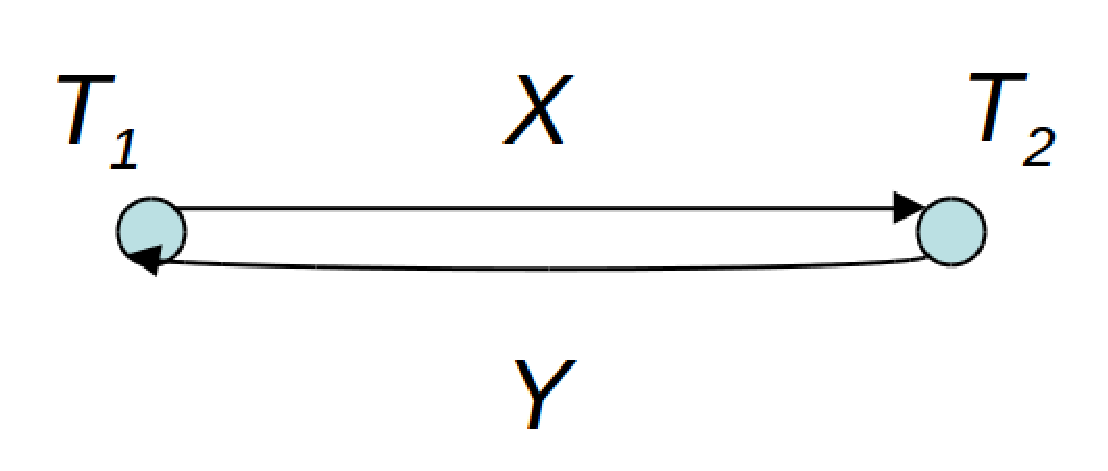
\includegraphics[width=170px]{grafo1.eps}\\
 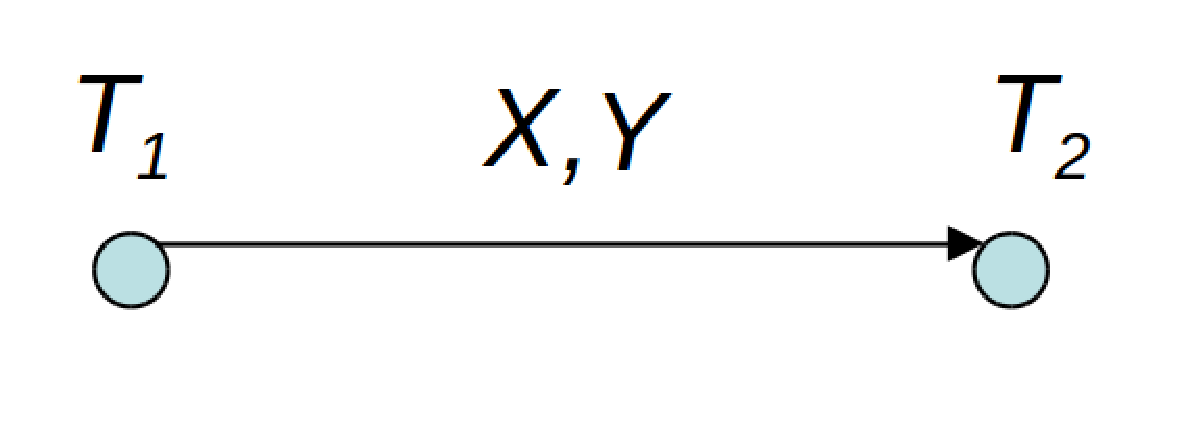
\includegraphics[width=170px]{grafo2.eps}
\end{multicols}

Considerando invece il seguente grafo, una possibile eliminazione ricorsiva dei nodi con archi non entranti
produce il seguente schedule seriale: $t_4$, $t_7$, $t_5$, $t_1$, $t_8$, $t_9$, $t_2$, $t_3$, $t_6$.\\
\begin{center}
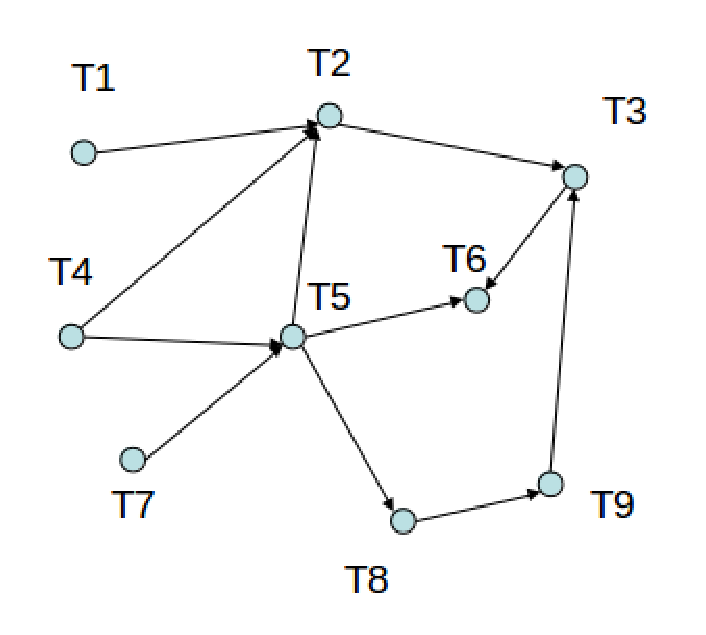
\includegraphics[width=200px]{ordinamento_topologico.eps}\\ 
\end{center}

\noindent Il seguente teorema prova la correttezza dell'algoritmo.
\label{teorema_6_1}
\begin{theo}
L'Algoritmo 1 determina correttamente se uno schedule è serializzabile. 
\end{theo}
\textbf{Dimostrazione.} Cominciamo con il dimostrare che se il grafo di serializzazione $G$ contiene un ciclo allora $S$
non è serializzabile. Supponiamo, per assurdo, che $G$ contenga un ciclo $t_1$, $t_2, \ldots, t_k$, $t_1$ e che
esista uno schedule seriale $S'$ equivalente ad $S$. Sia $t_i$, $1\leq i \leq k$, la transazione del ciclo che compare
per prima in $S'$ e sia $X$ l'item che causa la presenza in $G$ dell'arco da $t_i-1$ a $t_i$. Il valore finale per $X$
prodotto da $S'$ è dato da una formula in cui compare una funzione $f$ associata ad una coppia lockunlock
in $t_i-1$ e almeno uno degli argomenti di $f$ è una formula in cui compare una funzione $g$
associata ad una coppia lock-unlock in $t_i$. D'altra parte in $S$ l'effetto di $t_i-1$ su $X$ precede quello di $t_i$
su $X$ ; quindi nella formula che dà il valore finale per $X$ prodotto da $S$ la funzione f compare più
internamente di $g$ ($f$ è applicata prima di $g$). Pertanto $S'$ ed $S$ non sono equivalenti (contraddizione).
Mostriamo ora che se $G$ non ha cicli allora $S$ è serializzabile. A tal fine definiamo profondità di una
transazione $t$ la lunghezza del più lungo cammino in $G$ da un qualsiasi nodo a $t$.
Sia $S'$ lo schedule seriale costruito dall'algoritmo; mostreremo per induzione sulla profondità delle
transazioni che ogni transazione $t$ per ogni item su cui effettua un'operazione di lock legge in $S$ lo
stesso valore che legge in $S'$ (e quindi per ogni item su cui effettua un'operazione di lock produce in
$S$ lo stesso valore che produce in $S'$).
Base dell'induzione. Se per una transazione $t$ la profondità è 0 vuol dire che in $G$ non ci sono archi
entranti in $t$; pertanto in $S$ $t$ legge solo valori iniziali. D'altra parte in $S'$ $t$ viene prima di qualsiasi
transazione che effettua un'operazione di lock su un item su cui $t$ effettua un'operazione di lock.
Infatti, se $X$ è un item su cui $t$ effettua un'operazione di lock e $t_{i_1}, t_{i_2}, \ldots, t_{i_k}$ è la sequenza in $S$
delle transazioni che effettuano un'operazione di lock su $X$, $t_{i_1}, t_{i_2}, \ldots, t_{i_k}$ è un cammino in $G$;
poiché $t$ deve comparire in tale cammino e in $G$ non ci sono archi entranti in $t$, si deve avere $t=t_{i_1}$
e quindi nessun altro nodo del cammino può essere eliminato dal procedimento di ordinamento
topologico prima di $t$.
Induzione. Cominciamo con il mostrare che ogni transazione per ogni item su cui effettua
un'operazione di lock legge sia in $S$ che in $S'$ il valore prodotto da una stessa transazione.
Supponiamo, per assurdo, che esistano una transazione $t$ e un item $X$ tali che $t$ legge in $S$ il valore
di $X$ prodotto da una transazione $t'$ e in $S'$ il valore prodotto da un'altra transazione $t''$. Sia $t_{i_1},
t_{i_2}, \ldots, t_{i_k}$ la sequenza in $S$ delle transazioni che effettuano un'operazione di lock su $X$; $t_{i_1},
t_{i_2}, \ldots, t_{i_k}$ è un cammino in $G$ in cui $t'$ compare immediatamente prima di $t$. Anche $t''$ compare in tale
cammino, e quindi deve comparire prima di $t'$. Poiché in $S'$, $t''$ deve seguire $t'$, $S'$ non può essere
ottenuto da $G$ mediante il procedimento di ordinamento topologico (contraddizione).
Sia $t$ una transazione che ha profondità $d$, $d>0$, in $G$; per quanto visto $t$, per ogni item su cui
effettua un'operazione di lock, legge sia in $S$ che in $S'$ il valore prodotto da una stessa transazione
$t'$. Poiché $t'$ ha profondità minore di $d$ per l'ipotesi induttiva $t'$, per ogni item su cui effettua
un'operazione di lock, legge sia in $S$ che in $S'$ lo stesso valore e, quindi, produce sia in $S$ che in $S'$ lo
stesso valore. Pertanto $t$, per ogni item su cui effettua un'operazione di lock, legge sia in $S$ che in $S'$
lo stesso valore. \hfill $\Box$\\
\begin{defn}
Diciamo che una transazione obbedisce al protocollo di locking a due fasi, o più semplicemente che
è \textbf{a due fasi}, se prima effettua tutte le operazioni di lock (fase di locking) e poi tutte le operazioni di
unlock (fase di unlocking). 
\end{defn}
Mostreremo che il protocollo di locking a due fasi garantisce la serializzabilità; più precisamente, si ha che:
\begin{theo}
Sia $T$ un insieme di transazioni. Se ogni transazione in $T$ è a due fasi allora ogni
schedule di $T$ è serializzabile. 
\end{theo}
\textbf{Dimostrazione.} Sia $S$ uno schedule di $T$. Supponiamo, per assurdo, che $S$ non sia serializzabile. Per il
\linkto{teorema_6_1}{Teorema 6.1}, il grafo di serializzazione $G$ di $S$ contiene un ciclo $t_{i_1}, t_{i_2}, \ldots,
t_{i_k}$; ciò significa che $t_{i+1}$, $i\in \{1,\ldots k-1\}$, effettua un'operazione di lock, su un item su cui $t_i$
ha effettuato un'operazione di unlock e che $t_1$ effettua un'operazione di lock, su un item su cui $t_k$ ha effettuato
un'operazione di unlock. Pertanto in $S$ $t_1$ effettua un'operazione di lock dopo aver effettuato un'operazione di unlock
e quindi $t_1$ non è a due fasi (contraddizione).\\

Mostreremo ora che se una transazione $t_1$ non è a due fasi, esiste sempre una transazione $t_2$ tale
che esiste uno schedule di $\{t_1, t_2\}$ che non è serializzabile. Infatti, se $t_1$ non è a due fasi, effettua
un'operazione di lock dopo aver effettuato un'operazione di unlock; consideriamo anche la seguente transazione $t_2$  

\begin{multicols}{2}  

 \begin{tabular}{|l|}
   \hline
   $t_1$\\
   \hline
   $\ldots$\\
   unlock(X)\\ 
   $\ldots$\\
   lock(Y)\\ 
   $\ldots$\\
  \hline
 \end{tabular}
 
 \begin{tabular}{|l|}
  \hline
   $t_2$\\
   \hline
   lock(X)\\
   lock(Y)\\
   unlock(X)\\
   unlock(Y)\\
  \hline
  \end{tabular} 
 \end{multicols}
 

 il seguente schedule $S$ di $t_1$ e $t_2$ non è serializzabile
\begin{center}
 \begin{tabular}{|l|l|}
 \hline
 $t_1$ & $t_2$\\
 \hline
   $\ldots$&\\
   unlock(X)&\\
   $\ldots$&\\
   &lock(X)\\
   &lock(Y)\\
   &unlock(X)\\    
   &unlock(Y)\\
   $\ldots$&\\
   lock(Y)&\\
   $\ldots$&\\
   \hline
  \end{tabular}
\end{center}

Infatti il suo grafo di serializzazione
\begin{center}
  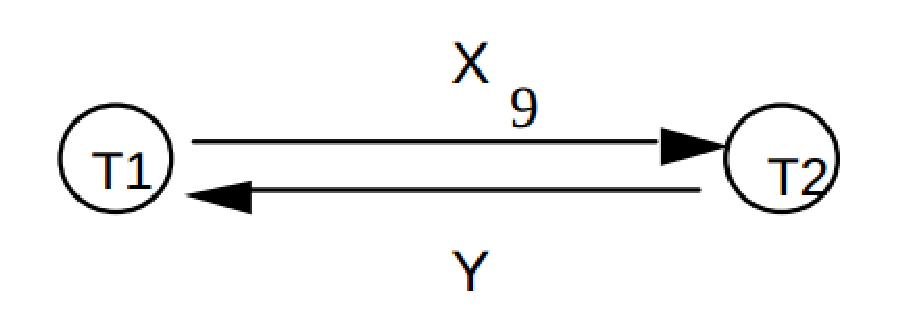
\includegraphics[width=150px]{img_6_3_1.eps}
\end{center}
contiene un ciclo. Naturalmente possono esistere schedule di transazioni che non sono a due fasi
che sono serializzabili. Tuttavia poiché è normale non conoscere l'insieme di transazioni con cui
una transazione può essere eseguita concorrentemente siamo costretti a richiedere che tutte le
transazioni siano a due fasi perché sia garantita la serializzabilità di ogni schedule.

\subsubsection{Lock a tre valori}
Consideriamo ora un modello per le transazioni che consente un maggior grado di concorrenza. In
tale modello si fa l'assunzione realistica che una transazione possa accedere ad un item solo per
leggerlo, senza modificarlo. Se una transazione desidera solo leggere un item $X$ effettua
un'operazione $rlock(X)$ che impedisce a qualsiasi altra transazione di modificare il valore di $X$;
tuttavia un qualsiasi numero di transazioni può ottenere contemporaneamente un lock di lettura su
$X$. Se, invece, una transazione desidera modificare il valore di $X$ effettua un'operazione $wlock(X)$; in
tal caso nessuna altra transazione può ottenere un lock di scrittura o di lettura su $X$. Entrambi i lock
sono rilasciati mediante un'operazione di $unlock(X)$. Pertanto si fa uso di un lock a tre valori:
$rlocked$, $wlocked$, $unlocked$.\\
Quanto detto per gli schedule legali vale anche in questo modello con l'unica differenza che una
transazione che mantiene un lock di lettura su un certo item può richiedere un lock in scrittura su
quello stesso item.\\
Analogamente a quanto fatto per il modello precedente assumiamo che quando una transazione
effettua un $wlock$ su un item il nuovo valore dell'item viene calcolato da una funzione,
univocamente associata a quell'operazione di $wlock$, che ha come argomenti tutti gli item su cui la
transazione ha già effettuato un lock (di lettura o di scrittura) prima dell'unlock associato al $wlock$.
Quindi, analogamente a quanto accadeva nel modello precedente, l'effetto di uno schedule sulla
base di dati può essere espresso dalle formule che calcolano (a partire dai valori iniziali degli item e
applicando le funzioni associate ai $wlock$) i valori degli item che sono modificati da almeno una
transazione. Tuttavia, poiché in questo modello si assume che una transazione possa leggere un item
senza modificarlo, la definizione di equivalenza di schedule deve essere modificata per tener conto
di tale eventualità.\\
\begin{defn}
 Due schedule sono \textbf{equivalenti} se:
 \begin{enumerate}
  \item producono lo stesso valore per ogni item su cui viene effettuato un wlock
  \item ogni operazione rlock(X) legge lo stesso valore di $X$ nei due schedule.
 \end{enumerate}
\end{defn}


Vediamo ora quali condizioni di precedenza tra transazioni è possibile inferire dalla semantica delle
transazioni appena vista.\\
Supponiamo che in uno schedule $S$ una transazione $t_1$ effettui un'operazione $wlock$ su un item $X$ e
che una transazione $t_2$ effettui un'operazione rlock su $X$ prima che una terza transazione $t_3$ esegua
la successiva operazione di $wlock$ su $X$ (in altre parole, $t_1$ modifica il valore di $X$ e $t_2$ legge il
valore di $X$ prodotto da $t_1$ prima che $X$ venga nuovamente modificato da $t_3$). Allora in qualsiasi
schedule seriale equivalente ad S $t_1$ deve precedere $t_2$ e $t_2$ deve precedere $t_3$. D'altra parte, se due
transazioni $t_1$ e $t_2$ leggono entrambe il valore di un item $X$ prodotto da una transazione non è lecito
stabilire nessuna precedenza tra $t_1$ e $t_2$ .
Per rappresentare le precedenze tra le transazioni è possibile usare, come per il modello precedente,
un grafo diretto che ha per nodi le transazioni e ha un arco da una transazione $t_i$ a una transazione
$t_j$ se la semantica delle transazioni impone che $t_i$ debba precedere $t_j$. Analogamente a quanto
accade per il modello precedente, un semplice algoritmo su tale grafo permette di decidere se uno
schedule è serializzabile e in caso affermativo di ottenere uno schedule seriale equivalente ad esso.

\begin{alg}
Dato uno schedule $S$
\begin{itemize}
 \item crea un grafo diretto $G$ (grafo di serializzazione) i cui nodi corrispondono alle transazioni; in
tale grafo c'è un arco diretto da $t_i$ a $t_j$ se
 \begin{itemize}
  \item in $S$ $t_i$ esegue una $rlock(X)$ o una $wlock(X)$ e $t_j$ è la transazione che esegue la successiva
   $wlock(X)$
  \item in $S$ $t_i$ esegue una $wlock(X)$ e $t_j$ esegue una $rlock(X)$ dopo che $t_i$ ha eseguito la $wlock(X)$ e
prima che un'altra transazione esegua una $wlock(X)$.
 \end{itemize}
\item verifica se $G$ ha un ciclo. Se $G$ ha un ciclo allora $S$ non è serializzabile; altrimenti esiste un
ordinamento $S'$ delle transazioni tale che $t_i$ precede $t_j$ se c'è in $G$ un arco diretto da $t_i$ a $t_j$; tale
ordinamento può essere ottenuto applicando a $G$ il procedimento di ordinamento topologico.
\end{itemize}
\end{alg}

Il seguente teorema, che può essere dimostrato con la stessa tecnica usata per il \linkto{teorema_6_1}{Teorema 6.1},
prova la correttezza dell'algoritmo.
\begin{theo}
L'Algoritmo 2 determina correttamente se uno schedule è serializzabile. 
\end{theo}

Consideriamo le seguenti transazioni:
\begin{multicols}{3}
 \begin{tabular}{|l|}
  \hline
  $t_1$\\
  \hline
  rlock(X)\\
  unlock(X)\\
  wlock(Y)\\
  unlock(Y)\\
  \hline
 \end{tabular}
 
  \begin{tabular}{|l|}
  \hline
  $t_2$\\
  \hline
  wlock(X)\\
  unlock(X)\\
  rlock(Z)\\
  unlock(Z)\\
  \hline
 \end{tabular}
 
  \begin{tabular}{|l|}
  \hline
  $t_3$\\
  \hline
  rlock(Y)\\
  unlock(Y)\\
  wlock(Z)\\
  unlock(Z)\\
  \hline
 \end{tabular}
\end{multicols}

Il seguente schedule di $\{t_1, t_2, t_3\}$ è serializzabile
\begin{center}
\begin{tabular}{|l|l|l|}
 \hline
 $t_1$ & $t_2$ & $t_3$\\
 \hline
 rlock(X)& &\\
 unlock(X)& &\\
 & wlock(X)& \\
 & unlock(X)& \\
 wlock(Y)& & \\
 unlock(Y)& &\\
 & & rlock(Y)\\
 & & unlock(Y)\\
 & &wlock(Z)\\
 & &unlock(Z)\\
 & rlock(Z)& \\
 & unlock(Z)& \\
\hline
 \end{tabular}
\end{center}

infatti il suo grafo di serializzazione

\begin{center}
 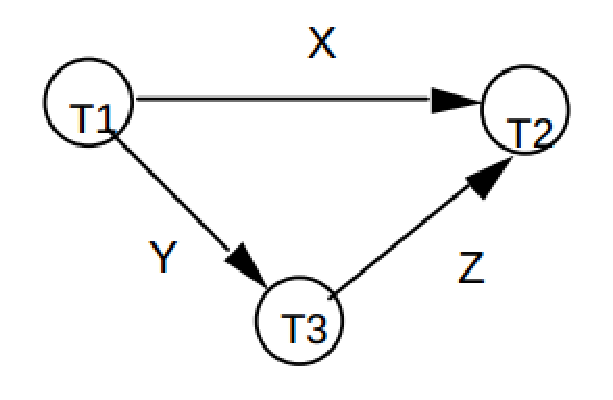
\includegraphics[width=150px]{grafo3.eps}
\end{center}

non contiene cicli; lo schedule seriale equivalente fornito dall’algoritmo è $t_1$, $t_3$, $t_2$. Al contrario il
seguente schedule di $\{t_1$, $t_2$, $t_3\}$ non è serializzabile

\begin{center}
\begin{longtable}{|l|l|l|}
 \hline
 $t_1$ & $t_2$ & $t_3$\\
 \hline
 rlock(X)& &\\
 unlock(X)& &\\
 & wlock(X)& \\
 & unlock(X)& \\
 & & rlock(Y) \\
 & & unlock(Y)\\
 & rlock(Z)& \\
 & unlock(Z)& \\
 & &wlock(Z)\\
 & &unlock(Z)\\
 wlock(Y) & &\\
 unlock(Y) & &\\
\hline
 \end{longtable}
\end{center}

infatti il suo grafo di serializzazione

\begin{center}
 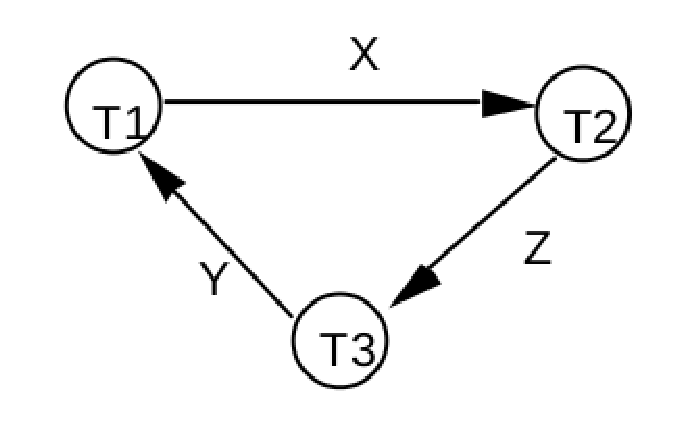
\includegraphics[width=150px]{img_6_3_2.eps}
\end{center}
contiene un ciclo.\\

Analogamente a quanto mostrato per il modello precedente anche per questo modello è possibile
dimostrare che qualsiasi schedule di un insieme di transazioni a due fasi (cioè transazioni in cui
nessuna operazione di lock può seguire una operazione di unlock) è serializzabile e che per qualsiasi
transazione $t$ a due fasi esiste uno schedule di transazioni contenente $t$ e almeno una transazione
non a due fasi che non è serializzabile.

\subsubsection{Read-only, write-only}
Nei due modelli di transazioni esaminati precedentemente viene fatta l'assunzione che ogni volta
che una transazione modifica un item $X$ legge il vecchio valore di $X$ e il nuovo valore di $X$ dipende
dal vecchio; in particolare nel primo modello l'insieme degli item letti e quello degli item scritti da
una transazione coincidono, mentre nel secondo modello l'insieme degli item scritti da una
transazione è contenuto nell'insieme degli item letti dalla stessa transazione. Un modello più
realistico dovrebbe prevedere che non ci sia necessariamente una relazione di contenimento tra
l'insieme degli item letti, \emph{read set}, e quello degli item scritti, \emph{write set}, da una transazione. Pertanto
considereremo ora un modello in cui, analogamente al modello precedente, una transazione può
effettuare operazioni di rlock e wlock, ma in cui:
\begin{enumerate}
 \item non si assume che quando una transazione scrive un item debba averlo letto
 \item non si assume che il valore di un item letto da una transazione sia significativo
indipendentemente dal fatto che abbia influenza sul valore finale di qualche item prodotto dalla
transazione.
\end{enumerate}
In conseguenza del punto 2, dovremmo considerare equivalenti due schedule se producono lo stesso valore
per ogni item su cui effettuano operazioni di scrittura. Una definizione di serializzabilità basata su
tale nozione di equivalenza non è però soddisfacente, come mostrato dall'esempio seguente.\\

Consideriamo lo schedule
\begin{center}
\begin{tabular}{|l|l|l|}
 \hline
 $t_1$ & $t_2$ & $t_3$\\
 \hline
 wlock(A)& &\\
 unlock(A)& &\\
 & wlock(C)& \\
 & unlock(C)& \\
 & rlock(A) & \\
 & rlock(B) &\\
  & unlock(A) &\\
  & unlock(B) &\\
 rlock(C) & &\\
 wlock(D) & &\\
 unlock(C)& & \\
 unlock(D)& & \\
 & & wlock(B)\\
 & & wlock(D)\\
 & & unlock(B)\\
 & & unlock(D)\\
\hline
 \end{tabular}
\end{center}


In base alla definizione di serializzabilità, detta \textbf{view serializability}, data sopra, tale schedule è
serializzabile; infatti i valori finali prodotti dallo schedule per gli item $A$, $B$, $C$ e $D$ sono i valori per
tali item calcolati rispettivamente dalle transazioni $t_1$, $t_3$, $t_2$ e $t_3$ e sono gli stessi valori prodotti
dallo schedule seriale $t_1$, $t_2$, $t_3$ . Tuttavia, se la transazione $t_3$ non viene eseguita (ad esempio per la
caduta del sistema) i valori finali prodotti per gli item $B$ e $D$ non coincidono né con i valori prodotti
dallo schedule seriale $t_1$, $t_2$, né con i valori prodotti dallo schedule seriale $t_2$, $t_1$.
Inoltre è stato dimostrato che se si adotta tale definizione di serializzabilità, il problema di decidere
se uno schedule è serializzabile risulta essere \emph{NP-completo}.\\
Prenderemo pertanto in esame un'altra definizione di serializzabilità, più restrittiva della
precedente, detta \textbf{conflict serializabilty}, basata su alcuni vincoli di precedenza imposti dalla
semantica delle transazioni; in base a tale definizione lo schedule appena visto risulta non
serializzabile.\\
Nel modello esaminato precedentemente se in uno schedule $S$ una transazione $t_1$ effettua un
$wlock(X)$ e $t_2$ è un'altra transazione che effettua il successivo $wlock(X)$ allora $t_2$ legge il valore di
$X$ scritto da $t_1$ e in base a tale valore calcola il nuovo valore di $X$; pertanto in qualsiasi schedule
seriale equivalente ad S $t_1$ deve precedere $t_2$ . Nel modello attualmente in esame, se $t_2$ non legge $X$
non c'è alcun motivo per cui debba seguire $t_1$ in uno schedule seriale equivalente ad $S$; in altre
parole due scritture successive di uno stesso item da parte di due distinte transazioni non
impongono nessun vincolo di precedenza. Vediamo quindi quali sono i vincoli che vanno
effettivamente imposti per uno schedule seriale equivalente ad uno schedule $S$:
\begin{enumerate}
 \item Se in $S$ una transazione $t_2$ legge il valore di un item $X$ scritto da una transazione $t_1$ allora $t_1$
deve precedere $t_2$ e,
 \item se $t_3$ è una terza transazione che scrive $X$ allora $t_3$ deve precedere $t_1$ o seguire $t_2$ .
\end{enumerate}
A tali vincoli devono essere aggiunti i seguenti:
\begin{enumerate}
\item se una transazione legge il valore iniziale di un item $X$ allora deve precedere qualsiasi
transazione che scriva $X$
\item se una transazione scrive il valore finale di un item $X$ allora deve seguire qualsiasi transazione
che scriva $X$.
\end{enumerate}

Se postuliamo l'esistenza all'inizio dello schedule di una transazione iniziale $t_0$ che scrive i valori
iniziali di tutti gli item (senza leggerne nessuno) e alla fine dello schedule di una transazione finale
$t_f$ che legge i valori finali di tutti gli item (senza scriverne alcuno), gli ultimi due vincoli sono
riassorbiti dal vincolo 1. Nel seguito dato uno schedule $S$ indichiamo con $S$ lo schedule ottenuto da
$S$ aggiungendo all'inizio la transazione iniziale e alla fine quella finale.\\

Diciamo allora che
\begin{defn}
 Uno schedule $S$ è serializzabile se esiste uno schedule seriale che rispetta tutti i
vincoli di tipo 1 e 2 generati da $S$.
\end{defn}

Analogamente a quanto visto per i modelli precedenti anche in questo caso possiamo rappresentare i
vincoli di precedenza imposti dalla semantica delle transazioni mediante gli archi in un particolare
tipo di grafo diretto. In particolare il vincolo 1 può essere rappresentato da un arco diretto $t_1\rightarrow t_2$ e
il vincolo 2 dalla coppia di archi alternativi $t_3\rightarrow t_1$ e $t_2\rightarrow t_3$. Una collezione di nodi, archi e
coppie di archi alternativi viene detta poligrafo. Un poligrafo è aciclico se almeno uno dei grafi che
possono essere ottenuti prendendo un arco da ogni coppia di grafi alternativi è aciclico.
Analogamente a quanto visto per i modelli precedenti, anche in questo caso la serializzabilità di uno
schedule può essere testata da un algoritmo che costruisce un poligrafo e quindi verifica se è
aciclico; inoltre, se è aciclico, fornisce (applicando l'ordinamento topologico ad un grafo aciclico
ottenuto dal poligrafo nel modo detto sopra) uno schedule seriale che rispetta i vincoli di
precedenza tra transazioni imposti dallo schedule dato. Prima di esaminare l'algoritmo osserviamo
che poiché in questo modello non si assume che il valore di un item letto da una transazione sia
significativo indipendentemente dal fatto che abbia influenza sul valore finale di qualche item
prodotto dalla transazione, una transazione che non ha alcun effetto sui valori finali prodotti da uno
schedule è considerata inutile in quello schedule. Come vedremo le transazioni inutili vengono
eliminate dall'algoritmo in quanto sono irrilevanti nel determinare la serializzabilità di uno schedule
(in altre parole una transazione inutile in uno schedule $S$ può leggere in $S$ e in uno schedule seriale
$S'$, che rispetta i vincoli di precedenza tra transazioni imposti da $S$, valori diversi).

\begin{defn}
Dato uno schedule $S$ i nodi del poligrafo $P$ sono le transazioni di $S$. 
\end{defn}

La costruzione degli archi di $P$ avviene attraverso i seguenti passi:
\begin{enumerate}
 \item vengono creati gli archi in accordo al vincolo 1; quindi se una transazione $t_2$ legge il valore di
un item $X$ scritto da una transazione $t_1$ viene aggiunto l'arco diretto $t_1\rightarrow t_2$
 \item vengono eliminati tutti gli archi entranti in transazioni inutili (una transazione inutile $t$ può
essere individuata facilmente perché non c'è nessun cammino in $P$ da $t$ a $t_f$)
 \item vengono creati gli archi in accordo al vincolo 2; quindi per ogni arco $t_1\rightarrow t_2$ se $t_3$ è transazione
distinta da quella iniziale che scrive un item che ha imposto l'esistenza dell'arco $t_1\rightarrow t_2$, si
aggiunge:
\begin{itemize}
 \item l'arco $t_2\rightarrow t_3$ se $t_1 = t_0$ e $t_2 \not= t_f$
 \item l'arco $t_3\rightarrow t_1$ se $t_2 = t_f$ e $t_1 \not= t_0$
 \item la coppia di archi alternativi $t_3\rightarrow t_1$ e $t_2\rightarrow t_3$ se $t_1 \not= t_0$ e $t_2 \not= t_f$.
\end{itemize}
\end{enumerate}

Si consideri il seguente schedule
\begin{center}
 \begin{longtable}{|l|l|l|l|}
  \hline
  $t_1$ & $t_2$ & $t_3$ & $t_4$\\
  \hline
  & rlock(A) & & \\
  rlock(A) & & & \\
  wlock(C) & & & \\
  unlock(C) & & & \\
  & & rlock(C) & \\
  wlock(B) & & & \\
  unlock(B)& & & \\
  & & & rlock(B)\\
  unlock(A) & & & \\
  & unlock(A)& &\\
  & & wlock(A)& \\
  & & & rlock(C)\\
  & wlock(D) & & \\
 & & & unlock(B)\\
  & &unlock(C)&\\
 & rlock(B) & & \\
  & & unlock(A)& \\
 & & & wlock(A)\\
 & unlock(B)& &\\
 & & & wlock(B)\\
 & & & unlock(B)\\
 & unlock(D) & &\\
   & & &unlock(C)\\
 & & & unlock(A)\\
\hline
 \end{longtable}
\end{center}
Le figure seguenti mostrano il poligrafo che viene costruito ai passi 1, 2 e 3 dell'algoritmo.
\begin{center}
\begin{figure}[h!]
\centering
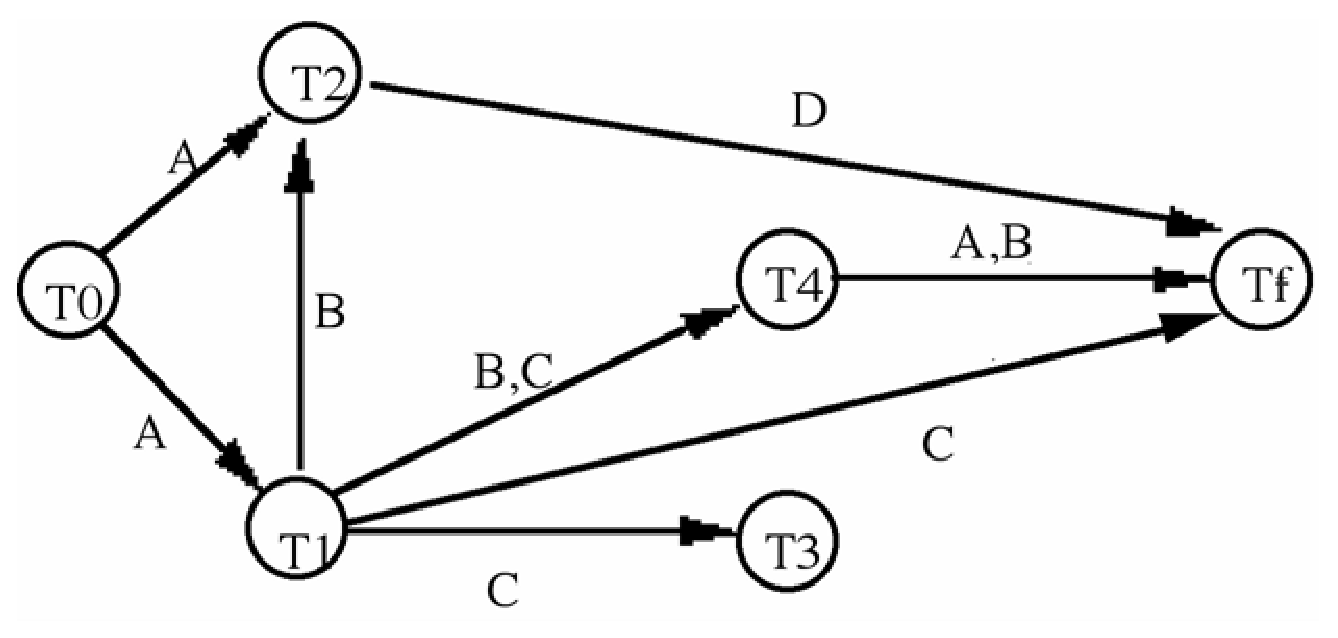
\includegraphics[width=200px]{img_6_3_2(1).eps}

Passo 1
\end{figure}

\begin{figure}[h!]
\centering
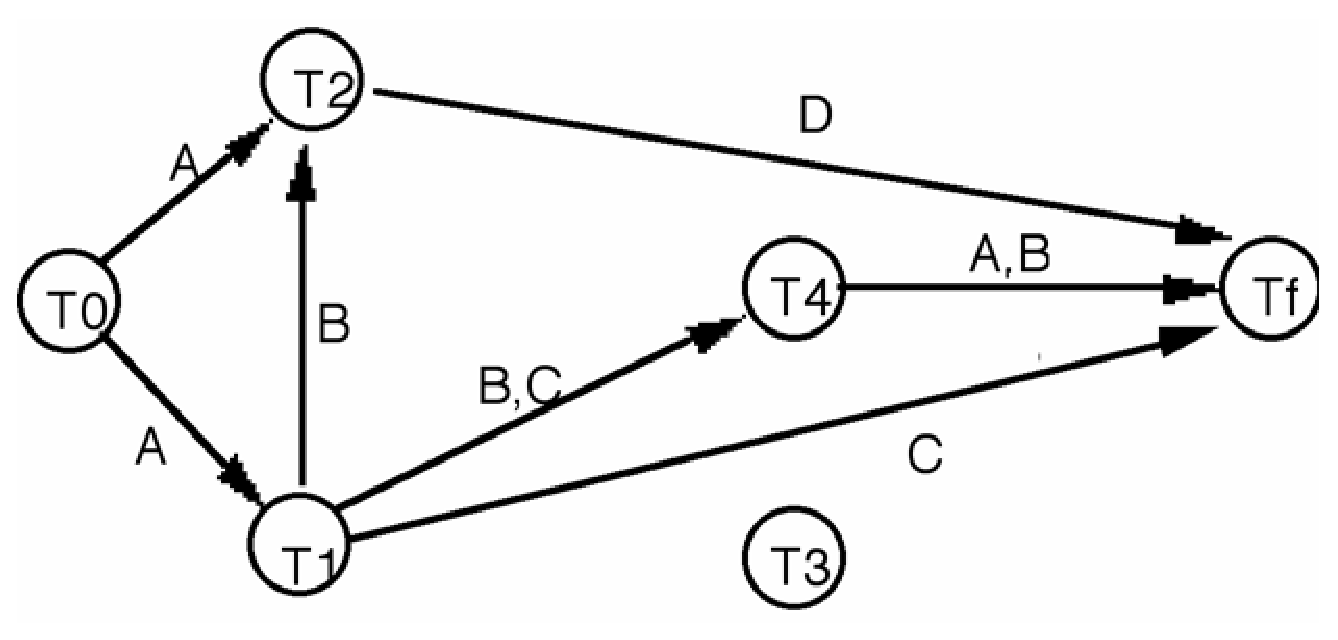
\includegraphics[width=200px]{img_6_3_2(2).eps}

Passo 2

\end{figure}

\begin{figure}[h!]
\centering
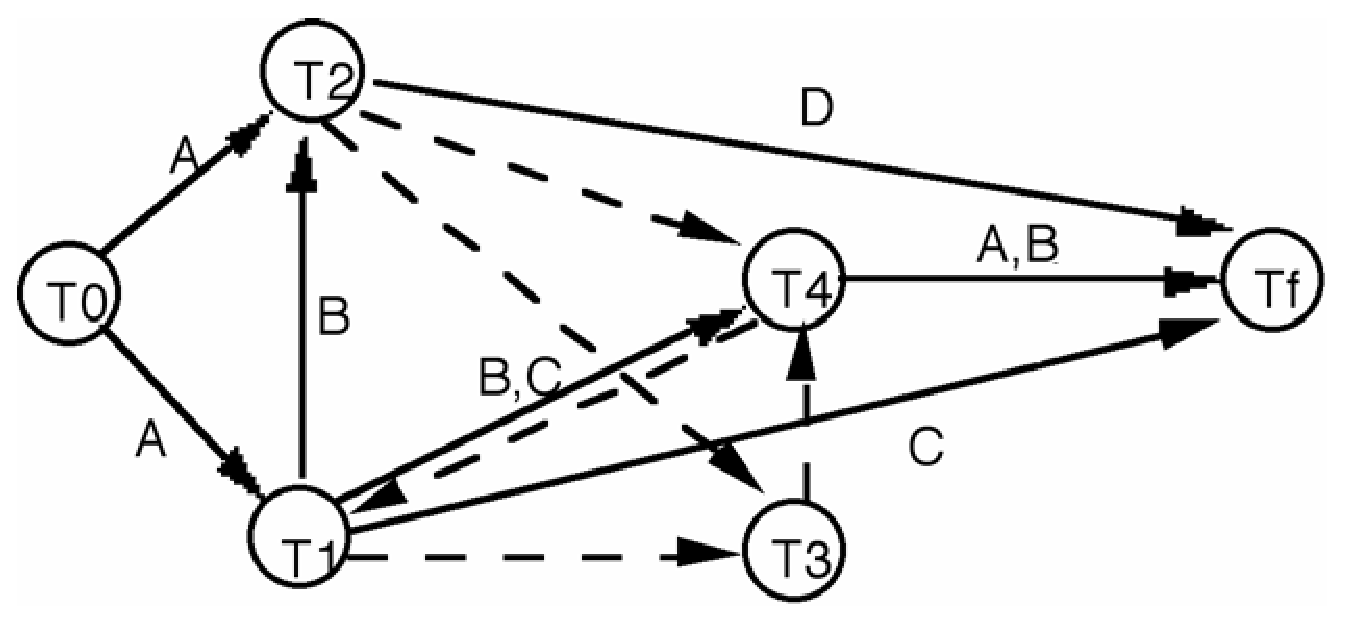
\includegraphics[width=200px]{img_6_3_2(3).eps}

Passo 3
\end{figure}
\end{center}

Poiché il poligrafo risultante è aciclico lo schedule è serializzabile e lo schedule seriale (che rispetta
i vincoli di precedenza tra transazioni imposti da esso) fornito dall'algoritmo è $t_1$, $t_2$, $t_3$,$t_4$.
Viceversa la figura seguente mostra il poligrafo costruito dall'algoritmo per lo schedule visto in
p recedenza; poiché contiene un ciclo, tale schedule non è serializzabile.
\begin{center}
 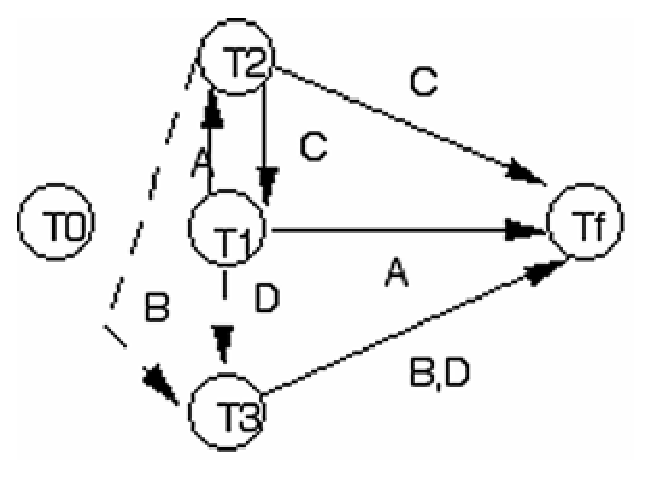
\includegraphics[width=150px]{img_6_3_2(4).eps}
\end{center}

\subsection{Deadlock e livelock}
In un sistema che utilizza i lock per il controllo della concorrenza si possono verificare delle
situazioni anomale note con il nome di \emph{deadlock} e \emph{livelock}.\\
Un \textbf{livelock} si verifica quando una transazione aspetta indefinitamente che gli venga garantito un
lock su un certo item. Ad esempio, consideriamo il caso di una transazione $t$ in attesa di effettuare
un lock su un item $X$ su cui un'altra transazione $t_1$ mantiene un lock; se quando $t_1$ rilascia $X$
un'altra transazione $t_2$ ottiene un lock su $X$, $t$ deve rimanere in attesa; poiché questa situazione può
ripeter si un numero indefinito di volte, $t$ può rimanere indefinitamente in attesa di ottenere un lock
su $X$.\\
Un \textbf{deadlock} si verifica quando ogni transazione in un insieme $T$ è in attesa di ottenere un lock su
un item sul quale qualche altra transazione in $t$ mantiene un lock.\\
Entrambi i problemi si possono presentare in un qualsiasi sistema in cui i processi possono essere
eseguiti concorrentemente e quindi sono stati largamente studiati nell'ambito dei sistemi operativi.
Il primo problema può essere risolto con una strategia first \emph{came-first served}; in altre parole il
sistema mantiene memoria delle successive richieste di lock in modo che, quando un item $X$ viene
rilasciato, viene garantito un lock su $X$ alla transazione che per prima ha richiesto un lock su $X$.
Un'altra possibile strategia può essere quella di eseguire le transazioni in base alle loro priorità e di
aumentare la priorità di una transazione all'aumentare del tempo in cui rimane in attesa in modo che
possa ad un certo punto assumere la priorità più alta ed essere eseguita.\\
Per risolvere il secondo problema possono essere seguiti due approcci. Un approccio è preventivo in
quanto cerca di evitare il verificarsi di situazioni di stallo adottando opportuni protocolli; l'altro
invece si preoccupa di risolvere le situazioni di stallo quando si verificano. Il sussistere di una
situazione di stallo può essere rilevato mantenendo un grafo di attesa, cioè un grafo i cui nodi sono
le transazioni e in cui c'è un arco $t_1$ →$t_2$ se la transazione $t_1$ è in attesa di ottenere un lock su un
item sul quale $t_2$ mantiene un lock; se in tale grafo c'è un ciclo si sta verificando una situazione di
stallo che coinvolge le transazioni nel ciclo; per risolverla occorre che almeno una transazione nel
ciclo sia \emph{rolled-back}. Una transazione è \textbf{rolled-back} quando viene abortita, 
i suoi effetti sulla base di dati vengono annullati ripristinando i valori dei dati precedenti 
l'inizio della sua esecuzione e, infine, tutti i lock mantenuti dalla transazione vengono rilasciati.
Una volta fatto ciò viene fatta ripartire.

\subsection{Protocollo di locking a due fasi stretto}
Oltre al verificarsi di un deadlock, ci sono altri motivi per cui una transazione deve essere abortita,
ad esempio perché ha cercato di effettuare un accesso non autorizzato oppure perché ha cercato di
eseguire una divisione per 0. Il punto in cui una transazione non può più essere abortita per uno dei
suddetti motivi, cioè il punto in cui ha ottenuto tutti i lock che gli sono necessari e ha effettuato tutti
i calcoli nell'area di lavoro, viene detto \textbf{punto di commit} della transazione; una transazione che ha
raggiunto il suo punto di commit viene detta \emph{committed} altrimenti viene detta \emph{attiva}. Quando una
transazione raggiunge il suo punto di commit effettua un'operazione di commit (nei sistemi reali
tale operazione prevede lo svolgimento di diverse azioni, ma per i nostri scopi serve solo a marcare
il punto di commit della transazione). I dati scritti da una transazione sulla base di dati prima che
abbia raggiunto il punto di commit vengono detti dati sporchi. Il fatto che un dato sporco possa
essere letto da qualche altra transazione può causare un effetto di roll-back a cascata.\\

Consideriamo il seguente schedule
\begin{center}
 \begin{longtable}{|l|l|}
 \hline
 $t_1$ & $t_2$\\
 \hline
wlock(X) & \\
read(X)& \\
$X\vcentcolon=X-N$& \\
write(X)& \\
unlock(X)& \\
 &rlock(X)\\
 &wlock(Z)\\
 &read(X)\\
 &read(Z)\\
 &$Z\vcentcolon=Z+X$\\
 &write(Z)\\
 &commit\\
 &unlock(X)\\
 &unlock(Z)\\
 wlock(Y)& \\
 read(Y)& \\
 $Y\vcentcolon=Y+N$& \\
 write(Y)& \\
 commit& \\
 unlock(Y)& \\
 \hline
 \end{longtable}
\end{center}

Se la transazione $t_1$ viene abortita dopo che ha letto $Y$, il valore di $X$ scritto da $t_1$ è un dato
sporco; infatti, quando $t_1$ viene abortita è necessario annullare gli effetti di $t_1$ sulla base di dati
ripristinando il vecchio valore di $X$ (quello letto da $t_1$). Ma allora è necessario annullare anche gli
effetti di $t_2$ sulla base di dati in quanto il valore di $Z$ prodotto da $t_2$ è calcolato a partire dal valore
di $X$ scritto $t_1$. Pertanto sia $t_1$ che $t_2$ devono essere rolled-back.\\
Per evitare questo fenomeno detto rollback a cascata occorre impedire alle transazioni di leggere
dati sporchi. Ciò può essere ottenuto adottando un protocollo di locking a due fasi stretto.
\begin{defn}
 Una transazione soddisfa il protocollo a due fasi stretto se:
 \begin{enumerate}
  \item non scrive sulla base di dati fino a quando non ha raggiunto il suo pun to di commit
  \item non rilascia un lock finchè non ha finito di scrivere sulla base di dati.
 \end{enumerate}
\end{defn}

La condizione 1 garantisce che se una transazione è abortita allora non ha modificato nessun item
nella base di dati; la condizione 2 garantisce che quando una transazione legge un item scritto da
un'altra transazione quest'ultima non può essere abortita (quindi nessuna transazione legge dati
sporchi).\\
Perché la transazione $t_1$ nell'esempio precedente soddisfi il protocollo di locking a due fasi stretto
deve essere modificata nel modo seguente.

\begin{center}
 \begin{tabular}{|l|}
  \hline
  $t_1$\\
  \hline
wlock(X)\\
read(X)\\
$X\vcentcolon=X-N$\\
wlock(Y)\\
read(Y)\\
$Y\vcentcolon=Y+N$\\
commit\\
write(X)\\
write(Y)\\
unlock(X)\\
unlock(Y)\\
\hline
 \end{tabular}
\end{center}

I protocolli di locking a due fasi stretti possono essere classificati in \emph{protocolli conservativi} e
\emph{protocolli aggressivi}; i primi cercano di evitare il verificarsi di situazioni di stallo, i secondi cercano
di processare le transazioni il più rapidamente possibile anche se ciò può portare a situazioni di
stallo e, quindi, alla necessità di abortire qualche transazione.\\

La versione più conservativa di un protocollo di locking a due fasi stretto è quella che impone ad
una transazione di richiedere all'inizio tutti gli item di cui può avere bisogno. Lo scheduler permette
alla transazione di procedere solo se tutti i lock che ha richiesto sono disponibili, altrimenti la mette
in una coda di attesa. In tal modo non possono verificarsi deadlock, ma possono ancora verificarsi
livelock. Per evitare anche il verificarsi di livelock si può impedire ad una transazione $t$ di
procedere (anche se tutti i lock da essa richiesti sono disponibili) se c'è un'altra transazione che
precede $t$ nella coda che è in attesa di ottene re un lock richiesto da $t$. \`E facile vedere che se si
adotta un protocollo in cui tutti i lock sono richiesti all'inizio e uno scheduler che garantisce ad una
transazione $t$ tutti i lock richiesti se e solo se:
\begin{enumerate}
 \item tutti i lock sono disponibili
 \item nessuna transazione che precede $t$ nella coda è in attesa di un lock richiesto da $t$
\end{enumerate}
allora non si possono verificare né dealdock né livelock. Infatti per la condizione 1 nessuna
transazione che mantiene un lock può essere in attesa di un lock mantenuto da un'altra transazione;
inoltre, la condizione 2 garantisce che dopo un tempo finito ogni transazione raggiunge la testa della
coda e quindi viene eseguita.\\

Il protocollo conservativo esaminato presenta due inconvenienti. Infatti l'esecuzione di una
transazione può essere ritardata dal fatto che non può ottenere un lock anche se molti passi della
transazione potrebbero essere eseguiti senza quel lock; inoltre una transazione è costretta a
richiedere un lock su ogni item che potrebbe essergli necessario anche se poi di fatto non l'utlizza.
Ad esempio, se una transazione deve effettuare una ricerca su un file con indice sparso e gli item
sono i blocchi, la transazione deve effettuare un lock su ogni blocco del file principale e del file
in dice anche se poi accederà soltanto ad alcuni blocchi del file indice e ad un solo blocco del file
principale.\\

La versione più aggressiva di un protocollo di locking a due fasi stretto è quella che impone ad una
transazione di richiedere un lock su un item immediatamente prima di leggerlo o scriverlo. Se le
transazioni soddisfano tale protocollo possono verificarsi situazioni di stallo; un modo per evitare
ciò è quello di definire un ordinamento sugli item e di imporre alle transazioni di richiedere i lock in
accordo a tale ordinamento. In tal modo non possono verificarsi deadlock. Infatti, sia $T$ un insieme
di transazioni (che richiedono i lock in accordo all'ordinamento fissato sull'insieme degli item) tale
che ogni transazione $t_k$ è in attesa di un item $A_k$ e mantiene un lock su almeno un item (si osservi
che se una transazione $t$ in $T$ non soddisfa la seconda condizione allora l'insieme $T-\{t\}$ è ancora
un insieme di transazioni in stallo) e sia $A$ i il primo item nell'ordinamento fissato sull'insieme degli
item; allora la transazione $t_i$ che è in attesa di $A_i$ non può mantenere un lock su alcun item
(contraddizione). Tuttavia il metodo di ordinare gli item non è molto praticabile perché non sempre
una transazione può scegliere l'ordine in cui richiedere i lock.\\
Un protocollo aggressivo è adatto a situazioni in cui la probabilità che due transazioni richiedano un
lock su uno stesso item è bassa (e quindi è bassa la probabilità che si verifichi una situazione di
stallo), in quanto evita al sistema il sovraccarico dovuto alla gestione dei lock (decidere se garantire
un lock su un dato item ad una data transazione, gestire la tavola dei lock, mettere le transazioni in
una coda o prelevarle da essa). Un protocollo conservativo è invece adatto a situazioni opposte in
quanto evita al sistema il sovraccarico dovuto alla gestione dei deadlock (rilevare e risolvere
situazioni di stallo, eseguire parzialmente transazioni che poi vengono abortite, rilascio dei lock
mantenuti da transazioni abortite).

\subsection{Controllo della concorrenza basato sui timestamp}
I metodi per il controllo della concorrenza basati sui \emph{timestamp} ordinano le transazioni in base ai
loro timestamp. Il timestamp è assegnato ad una transazione dallo scheduler quando la transazione
ha inizio. A tale scopo lo scheduler può o gestire un contatore (ogni volta che ha inizio una
transazione ta le contatore viene incrementato e il suo valore è il timestamp della transazione)
oppure usare l'orologio interno della macchina (in tal caso il timestamp è l'ora di inizio della
transazione).\\
In tale approccio al controllo della concorrenza, uno schedule è serializzabile se è equivalente allo
schedule seriale in cui le transazioni compaiono ordinate in base al loro timestamp.\\
Dato uno schedule occorre verificare che, per ciascun item acceduto da più di una transazione,
l'ordine con cui le transazioni accedono all'item non viola la serializzabilità dello schedule. A tale
sco po vengono associati a ciascun item $X$ due timestamp:
\begin{itemize}
 \item il read timestamp di $X$, denotato con $read\_TS(X)$, che è il più grande fra tutti i timestamp di
transazioni che hanno letto con successo $X$;
 \item il write timestamp di $X$, denotato con $write\_TS(X)$, che è il più grande fra tutti i timestamp di
transazioni che hanno scritto con successo $X$.
\end{itemize}

Ogni volta che una transazione $t$ cerca di eseguire un $read(X)$ o un $write(X)$, occorre confrontare il
timestamp $TS(t)$ di $t$ con il read timestamp e il write timestamp di $X$ per assicurarsi che l'ordine
basato sui timestamp non è violato. L'algoritmo per il controllo della concorrenza opera nel modo
seguente:
\begin{enumerate}
 \item ogni volta che una transazione $t$ cerca di eseguire l'operazione $write(X)$:
 \begin{enumerate}[a)]
  \item se $read\_TS(X) > TS(t)$, $t$ viene rolled back; infatti in tal caso qualche transazione con un
timestamp maggiore di $TS(t)$ (cioè una transazione che segue $t$ nell'ordinamento basato sui
timestamp) ha già letto il valore di $X$ prima che $t$ abbia potuto scriverlo, violando in tal
modo l'ordinamento basato sui timestamp;
 \item se $write\_TS(X) > TS(t)$, l'operazione di scrittura non viene effettuata; infatti in tal caso
qualche transazione $t'$ con un timestamp maggiore di $TS(t)$ (cioè una transazione che segue
$t$ nell'ordinamento basato sui timestamp) ha già scritto il valore di $X$ e quindi l'esecuzione
dell'operazione di scrittura provocherebbe la perdita di tale valore; si noti che nessuna
transazione $t''$ con $TS(t') > TS(t'') > TS(t)$, può aver letto $X$ altrimenti al passo precedente $t$
sarebbe stata rolled back;
\item se nessuna delle condizioni precedenti è soddisfatta allora l'operazione di scrittura è eseguita
e $TS(t)$ diventa il nuovo valore di $write\_TS(X)$
\end{enumerate}

\item ogni volta che una transazione $t$ cerca di eseguire l'operazione $read(X)$:
 \begin{enumerate}[a)]
\item se $write\_TS(X) > TS(t)$, $t$ viene rolled back; infatti in tal caso qualche transazione con un
timestamp maggiore di $TS(t)$ (cioè una transazione che segue $t$ nell'ordinamento basato sui
timestamp) ha già scritto il valore di $X$ prima che $t$ abbia potuto leggerlo, violando in tal
modo l'ordinamento basato sui timestamp;
\item se $write\_TS(X) \leq TS(t)$, allora l'operazione di lettura è eseguita e se $read\_TS(X) < TS(t)$,
$TS(T)$ diventa il nuovo valore di $read\_TS(X)$.
\end{enumerate}
\end{enumerate}

\noindent Consideriamo ad esempio le due transazioni seguenti
\begin{multicols}{2}
 \begin{tabular}{|l|}
  \hline
  $t_1$\\
  \hline
  read(X)\\
  $X\vcentcolon=X+10$\\
  write(X)\\
  \hline
 \end{tabular}

  \begin{tabular}{|l|}
  \hline
  $t_2$\\
  \hline
  read(X)\\
  $X\vcentcolon=X+5$\\
  write(X)\\
  \hline
 \end{tabular} 
\end{multicols}

con i seguenti timestamp: $TS(t_1)= 110$, $TS(t_2)=100$. Consideriamo il seguente schedule di $\{t_1, t_2\}$
\begin{center}
 \begin{tabular}{|l|l|}
 \hline
  $t_1$ & $t_2$\\
 \hline
 &read(X)\\
 read(X)&\\
 &$X\vcentcolon=X+5$\\
 $X\vcentcolon =X+10$&\\
  write(X)&\\
  &(*)write(X)\\
  \hline
 \end{tabular}
\end{center}

Quando $t_2$ cerca di eseguire $(*)$ viene abortita.\\

\noindent Consideriamo ora le due transazioni seguenti

\begin{multicols}{2}
 \begin{tabular}{|l|}
  \hline
  $t_1$\\
  \hline
  read(Y)\\
  $X\vcentcolon=Y+10$\\
  write(X)\\
  \hline
 \end{tabular}

  \begin{tabular}{|l|}
  \hline
  $t_2$\\
  \hline
  read(Y)\\
  $X\vcentcolon=Y+5$\\
  write(X)\\
  \hline
 \end{tabular} 
\end{multicols}
con i seguenti timestamp: $TS(t_1)= 110$, $TS(t_2)=100$. Consideriamo il seguente schedule di $\{t_1, t_2\}$
\begin{center}
 \begin{tabular}{|l|l|}
 \hline
  $t_1$ & $t_2$\\
 \hline
 &read(Y)\\
 read(Y)&\\
 &$X\vcentcolon=Y+5$\\
 $X\vcentcolon =Y+10$&\\
  write(X)&\\
  &(*)write(X)\\
  \hline
 \end{tabular}
\end{center}

In questo caso l’operazione $(*)$ non viene eseguita.
